\section{The Paṇḍaka}

\subsection{The Paṇḍaka in the Pali Vinaya}
In the Theravāda Vinaya the term {\em paṇḍaka} is mainly used in the context of individuals a monastic should not have sexual relations with or as a form of insult. The rule regarding the ordination of {\em paṇḍakas} is laid down in {\em Khandhaka 1}\footnote{Khandhaka 1 Pabbajjā PTS vol 1 page 85–86.} and reads as follows:\footnote{Translation by Ajahn Brahmali.}

\begin{quote}
{\em Tena kho pana samayena aññataro paṇḍako bhikkhūsu pabbajito hoti. So dahare dahare bhikkhū upasaṅkamitvā evaṃ vadeti—“etha, maṃ āyasmanto dūsethā”ti. Bhikkhū apasādenti—“nassa, paṇḍaka, vinassa, paṇḍaka, ko tayā attho”ti. So bhikkhūhi apasādito mahante mahante moḷigalle sāmaṇere upasaṅkamitvā evaṃ vadeti—“etha, maṃ āvuso dūsethā”ti. Sāmaṇerā apasādenti—“nassa, paṇḍaka, vinassa, paṇḍaka, ko tayā attho”ti. So sāmaṇerehi apasādito hatthibhaṇḍe assabhaṇḍe upasaṅkamitvā evaṃ vadeti—“etha, maṃ āvuso dūsethā”ti. Hatthibhaṇḍā assabhaṇḍā dūsesuṃ. Te ujjhāyanti khiyyanti vipācenti—“paṇḍakā ime samaṇā sakyaputtiyā. Yepi imesaṃ na paṇḍakā, tepi ime paṇḍake dūsenti. Evaṃ ime sabbeva abrahmacārino”ti. Assosuṃ kho bhikkhū tesaṃ hatthibhaṇḍānaṃ assabhaṇḍānaṃ ujjhāyantānaṃ khiyyantānaṃ vipācentānaṃ. Atha kho te bhikkhū bhagavato etamatthaṃ ārocesuṃ. “Paṇḍako, bhikkhave, anupasampanno na upasampādetabbo, upasampanno nāsetabbo”ti.}
\end{quote}

\begin{quote}
At one time a certain {\em paṇḍaka} had gone forth as a monk. He approached the young monks and said, “Venerables, come and have sex with me.” The monks dismissed him, “Go away, {\em paṇḍaka}. Who needs you?”

He went to the big and fat novices, said the same thing, and got the same response.

He then went to the elephant keepers and horse keepers, and once again he said the same thing. And they had sex with him. They complained and criticized them, “These Sakyan ascetics are {\em paṇḍakas}. And those who are not have sex with them. None of them is celibate.”

The monks heard their complaints. They told the Buddha and he said, “A {\em paṇḍaka} should not be given the full ordination. If it has been given, he should be expelled.”
\end{quote}

There are a couple of interesting things to note about this passage. First of all, the {\em paṇḍaka} in question was already ordained at the time of this incident. The rule against ordination of {\em paṇḍakas} clearly mentions that full ordination of these individuals, the {\em upasampadā}, is not allowed. This really only makes sense if we understand {\em pabbajjā} here to be equivalent to {\em upasampadā}. In fact this equivalence between {\em pabbajjā} and {\em upasampadā} is what we find throughout the earliest Vinaya, and indeed the suttas.\footnote{The {\em sāmaṇeras/īs} are barely mentioned in the suttas. Instead we find the figure of the {\em samaṇuddesa}, `one designated as a {\em samaṇa}', who seems to have had a looser affiliation with the {\em Saṅgha}, that is, no proper ordination. The commentaries glosses them as {\em sāmaṇeras}, but this might be an oversimplification. More likely they were a kind of precursor to the more formal status of novice. It seems likely that such people merely put on robes, and then lived in with loose connection to a particular community of ascetics, in which case their sex would have been a non-issue. I would argue it is natural to see novices proper in the same way. But the {\em samaṇuddesa} remains obscure.} In any case, the rule itself is clearly limited to {\em upasampadā} (full ordination) and novice ordination seems to be allowed.

The Theravāda commentary, both in regards to the {\em paṇḍaka} and the {\em ubhatob­yañ­janaka} differs from the Vinaya in making a distinction between {\em pabbajjā} (in the meaning of novice ordination) and {\em upasampadā} (full ordination) and does not allow either for ordination.

A second interesting point is that the monks and novices that are approached by the {\em paṇḍaka} react in an exemplary manner and send him away. It is only the elephant and horse keepers, those of a lower class, who engage in sexual relations with him. But afterwards, they still complain about it and criticize the {\em paṇḍaka} while they have themselves also engaged in the same act. This seems a bit odd and revolves around the stock passage {\em Te ujjhāyanti khiyyanti vipācenti} that is used throughout the Vinaya as a typical pattern of narration. In the majority of cases it is the {\em manussā} (people) who complain and criticize, after which the monks hear about it, also complain and criticize ({\em Ye te bhikkhū appicchā …pe… te ujjhāyanti khiyyanti vipācenti}) and then relate the story to the Buddha. So the word {\em te} (they) is used to relate to the monks who criticize after they have heard it from the `people'. Here however the word {\em te} is used right after the elephant and horse keepers, seemingly referring to them. However, it would make much more sense if others would complain about this scandalous behavior rather than the elephant and horse keepers themselves. Indeed this is what we find in the same story in the Dharmaguptaka Vinaya, where the people (lay Buddhists) complain and criticize (時諸居士見已譏嫌言). Claire Maes\footnote{See \cite{maes2011} pages 98–101.} points out that this phrase could have been used to conceal debates that might have influenced the Bhikkhu {\em Saṅgha} to implement specific precepts to be in conformity with the praxes of other ascetic communities with the main purpose to place the origin of precepts within the Buddhist Order with the Buddha himself in a leading role. She successfully demonstrates this with the Jain concept of {\em ekindriya jīva} (one-facultied life) and argues that this concept entered the Buddhist Vinaya as a result of interactions and discussions with the Jain contemporaries. I believe that the term {\em paṇḍaka} could also have entered the Buddhist Vinaya in a similar manner. As we have seen previously, the position of the {\em paṇḍaka} was discussed at length in the debate amongst the Jains themselves.

In Appendix \ref{appendix2}, figures \ref{pali1} and \ref{sanskrit1} I have charted the occurrences of the various words throughout the Pali and Sanskrit texts. This illustrates that the term {\em paṇḍaka} only occurs in the Vinaya and Commentaries in the Pali. The Sanskrit texts in this graph are not entirely organised by lateness but it is clear that the term {\em paṇḍaka} mainly appears in the Vinaya and {\em Śāstrapiṭaka}. The term {\em klība} is notable by it's absence in all Buddhist texts and only appears in the Vedic and later Brahmanical texts. It does not appear in the Pali texts at all. One explanation for this might be that the terms {\em klība} and {\em paṇḍaka} have been mixed up because their meanings were at least in part overlapping. What is also striking is that the umbrella term {\em napuṃsaka} only appears in the Pali commentarial texts and not in any of the earlier collections. It is however a recurrent term in the Vedic and Brahmanical texts. We also see that this term becomes more prominent in the later Anya commentaries as well as in the Brahmanical {\em Śāstra} collections, which points to a shift in emphasis, and possibly meaning, of this term in later times at the expense of the prominence of the term {\em paṇḍaka}. As these are later texts I have not looked into them in great details and this might be an interesting topic for later studies.

Considering that the word {\em paṇḍaka} does not appear in any of the early suttas\footnote{The word is not found in any of the early Buddhist Suttas, nor does it appear in the {\em pātimokkhas}, the lists of rules for monastics. Next to the Pali Vinaya, it appears twice in the {\em Aṅguttara Nikāya}, but both of these only have parallels to the Vinaya or later texts.}, it seems clear that the inclusion of the word in the Vinaya did not happen in the Buddha's lifetime but was added later as a result of the discussions with the Brahmins and Jains, for whom {\em paṇḍakas} could not ordain.

\subsection{The Five Types of Paṇḍaka}
Going beyond the Vinaya itself into the commentarial scriptures, we find the following in the Theravāda {\em Mahāvagga-aṭṭhakathā} to explain more about the nature of these two classes.\footnote{The {\em Samantapāsādikā}: Vol. V, p. 1015f. is a translation of Sinhala commentaries into Theravāda by Bhikkhu Buddhaghosa and possibly others in the 5\textsuperscript{th} Century CE. It was based on the Mahāpaccariya and the Kurundī Atthakathā. See \cite{goonesekere} for details on Theravāda Commentaries.} It defines five types of {\em paṇḍakas}:\footnote{Translations/explanations as in \cite{bomhard} and \cite{thanissaro}.}

\begin{enumerate}
\item {\em āsittapaṇḍaka}: a man who gains satisfaction from performing oral sex on another man and from swallowing his semen or who only becomes sexually aroused after swallowing another man’s semen. 
\item {\em usūyapaṇḍaka}: a voyeur, that is, a person who gains sexual satisfaction from watching others have sex. 
\item {\em opakkamikapaṇḍaka}: eunuch, due to castration.
\item {\em pakkhapaṇḍaka}: those who become sexually aroused in parallel with the phases of the moon.\footnote{According to \cite{bomhard}, the term pakkhapaṇḍaka (Skt. {\em pakṣapaṇḍaka}) probably does not refer, as traditionally understood, to an individual who becomes sexually aroused parallel to the phases of the moon, i.e., to someone who is aroused during the fortnight of either the waxing or waning moon, but to someone “who acts wrongly sexually, who behaves badly sexually.” He hypothesizes that {\em pakkha} of the compound {\em pakkhapaṇḍaka} should be understood in terms of its alternative meaning “a cripple,” and that the corresponding Sanskrit should not be understood as {\em pakṣa} but rather {\em phakka} (“cripple,” adj. “lame, crippled, maimed”), derived from the Skt. verbal root {\em phakk}, (a) “to creep, to steal along; (b) to have a preconceived opinion; (c) to act wrongly, to behave badly.” He thus considers the third meaning of phakk as most relevant to the case at hand.}
\item {\em napuṁsakapaṇḍaka}: a person born without sexual organs.\footnote{The Sanskrit equivalent is {\em prakṛtipaṇḍaka}. The term {\em prakṛti} means something like `nature' or `fundamental form' and the term {\em tṛtīyāprakṛti} became the official word for the `third sex' at around the beginning of the common era. I therefore do not believe this translation by \cite{thanissaro} to be correct but that the literal meaning reflects more the original meaning of {\em napuṁsaka}.} 
\end{enumerate}

It is interesting to note that not all {\em paṇḍakas} are barred from ordination, in contrast to what the Vinaya mentions. Only the last three types are forbidden to ordain.\footnote{\cite{wong} and \cite{thanissaro}.}

The castrated {\em paṇḍaka} i.e. a eunuch, is only one of the five types that cannot ordain, which makes it highly unlikely that the word {\em paṇḍaka} means `eunuch'. We would also not expect a eunuch to have hyperlibidinous-ness. After all, castrated men were often employed as harem guards just for the reason that they are no longer interested in sexual activity and therefore considered safe. Moreover, the Dharmaguptaka Vinaya treats the castrated man as something other than a {\em paṇḍaka}.

As we have seen in the Jain scriptures, the discussion to overcome the ambiguities in the understanding of the word {\em napuṁsaka} resulted over time in changes in meaning and the definition of sub-categories and I believe this has also occured in the Buddhist Vinayas with the word {\em paṇḍaka}. I believe that it is likely that the term {\em opakkamikapaṇḍaka} represented a castrated man, the {\em klība}, while the {\em napuṁsakapaṇḍaka} was the re-definition of the original {\em paṇḍaka} or the `female {\em napuṃsaka}' that we saw emerging in the Jain commentarial texts. Also from the Chinese sources it is clear that the person has to be born this way.

The {\em pakkhapaṇḍaka} is interesting and several explanations have been given by authors over time, none of which I find convincing. Allan \cite{bomhard} advocates that the word {\em pakkha} should not be translated as `half moon' but that the meaning of the word is something like a sex-addict. I refute this argument because the characters used to denote this type of pandaka in the Chinese Vinayas of all schools are 半月, which literally means `half moon'. It is also mentioned in various Chinese commentarial texts\footnote{f.i. X44 0744 0432c17 四分律名義標釋.} that the `half moon' is `not a male' and thus a form of {\em napuṃsaka} for half of the month and the other half he is a male. All texts are consistent in this. As we can still understand the meaning of the other four categories and understand their meaning in light of people's physiology or sexual fetishes, the `half-moon' {\em paṇḍaka} is an enigma. Turning back to the Vedic texts however, we find in the {\em Uttarakanda} of the {\em Rāmāyaṇam}\footnote{Rām 7.78–79. See also \cite{goldman} page 379–380.} the story of King Ila. In this epic tale the king accidentally stumbles upon the Goddess Pārvatī in intimate embrace with Śiva, who turn him into a woman. Now Ilā, she turns to the Goddess for mercy to restore her manhood but is only granted half her wish, namely that she has to change sex each month. The theme of changing genders based on the phases of the moon is a recurrent theme in the Vedic myths and it is not unlikely that this mythical theme has found its way into the Vinaya in the form of the {\em pakkhapaṇḍaka}. After all, another rule in the Vinayas of all the schools tells the tale of a shape-shifting serpent, a mythological beast, a {\em Nāga}\footnote{Khandhaka 1 Pabbajjā PTS vol 1 page 86–88.}, who ordains as a monk, is later discovered and a new rule is laid down in much the same manner as for the {\em paṇḍaka}, barring him and all his kind from ordination. The fabric of myth and reality can easily overlap in Indic culture. The Vinaya is full of various strange and wonderful beings. The ­{\em Bhikkhu Pā­rāji­ka} 1, the rule against sexual intercourse, mentions that a monk is not allowed to have sex with a list of beings, namely a dragon, a spirit, a ghost and a {\em paṇḍaka}.\footnote{PTS vol. 3 page 37: {\em Tena kho pana samayena aññataro bhikkhu nāgiyā methunaṃ dhammaṃ paṭisevi … yakkhiniyā methunaṃ dhammaṃ paṭisevi … petiyā methunaṃ dhammaṃ paṭisevi … paṇḍakassa methunaṃ dhammaṃ paṭisevi. Tassa kukkuccaṃ ahosi … pe … “āpattiṃ tvaṃ, bhikkhu, āpanno pārājikan”ti.}} The fact that the {\em paṇḍaka} is listed in a list of mythological beings is indicative of its origins and how they were viewed at that time. We find similar lists in the Vinayas of the other schools.

As for the other two, the {\em āsittapaṇḍaka} and the {\em usūyapaṇḍaka}, who at least in the Theravāda tradition are allowed to ordain, I believe they embody another of the Jain categories, namely the category of the {\em puruṣanapuṃsaka} (male {\em napuṃsaka}). Although they might be impotent and are therefore also in possession of the female {\em veda}, their appearance is male to the lay supporters but also to the celibate monks they live with who are not aroused by their presence. The relaxation of the rules for these two types also runs parallel with the development in the Jain scriptures. But unlike the Jain, no further abolishment of this entire rule against the ordination of {\em paṇḍakas} was reached simply because the Buddhist scriptures were closed while the Jain scriptures continued to evolve for many centuries thereafter.


\subsection{The Paṇḍaka in the Chinese Vinayas}
The first thing that is striking when comparing the various Chinese schools is that there is no clear consistent term that denotes the {\em paṇḍaka}. The Mahāsaṅghika and Sarvāstivāda Vinaya use the term 種不能男 (impotent lit. incapable of producing seed) in the descriptions in the first Khandhaka on ordination. In the Dharmaguptaka Vinaya this term is only used in the description of the `half-moon' {\em paṇḍaka}. The term 黃門 (`eunuch') is used in the Dharmaguptaka and Mahīśāsaka Vinaya while in the Sarvāstivāda Vinaya the term is used everywhere but in the ordination Khandhaka. As both the terms 種不能男 (impotent) and 黃門 (`eunuch') are used in the same way in different schools, we can assume that both can denote {\em paṇḍaka} but that the difference in terms point to historical changes in understanding and translation.\footnote{Shinsan text X44 0744 0432c13 (四分律名義標釋 第4卷) 0432c09–0433a01 links both terms: there are 5 types of 黃門 (lit. yellow gate)and 6 types of 種不能男 (i.e. seed incapable men), the 6\textsuperscript{th} type being those born from a concubine.}

The translation `eunuch' is a later interpolation due to the etymological development of the Chinese 黃門, meaning `yellow gate' and derived from the palace eunuchs in the Early Han Dynasty,\footnote{The word 黃門 is translated as `eunuch' but the characters spell a different word, namely `yellow gate'. The etymology of the word can be traced back to the Han Dynasty. See Shinsan text X44 0744 0432c09–0433a01: 此翻黃門。阿毗曇。譯為閹人。以無男根故。``This is a 黃門. Translated as castrated man. Because he has no male roots/faculty.'' This tells the story of the imperial ruler who appointed eunuchs to work for him. Yellow is the color of the middle in the `Five Directions' and of the earth in the `Five Elements' and therefore stands for imperial power and state. The color is only used by the emperor and others are not allowed to wear it. Therefore, the palace of the emperor is called the `Yellow Gate'. In the Easter Han Dynasty, the emperor hired eunuchs and they held rather powerful positions as palace guards, scribes and other official functions. They were called the `yellow gates'. It is a long story but the eunuchs became very powerful and eventually caused the downfall of the Han Dynasty (see \href{https://en.wikipedia.org/wiki/Han_dynasty}{Wikipedia}). So `yellow gate' became a synonym for `eunuch'.} while the word `impotent' seems to be an earlier interpretation and we also find this back in in the Vedic scriptures.\footnote{see \cite{zwilling} page 363–364.} The Chinese culture was vastly different from the ancient Indian culture and I suspect that their own palace eunuchs were the only thing they could relate to as an explanation of the term {\em paṇḍaka}.

The following table compares the description of the various schools, adding the Sanskrit\footnote{Abhidharmakośavyākhyā-Skt: 94, 15–25.} and Tibetan.\footnote{Abhidharmakośavyākhyā-Tib: D, vol. gu, 85b6–86a3; P, vol. cu, 97b2–7.} for reference\footnote{See \href{http://www.itlr.net/hwid:281142}{itlr.net} for details as well a more complete listing of possible meanings and occurrences of these terms.}

\bigskip
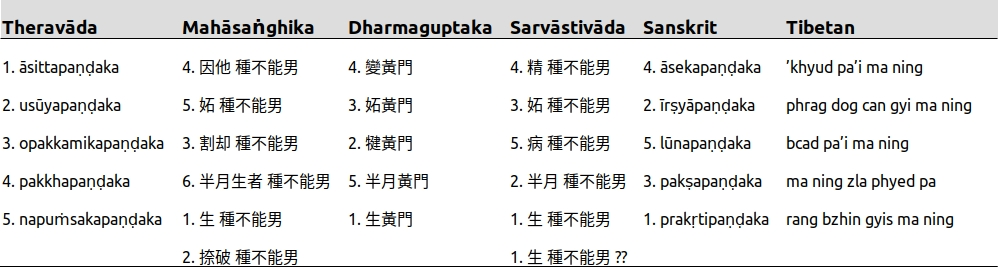
\includegraphics[width=\linewidth]{pandaka.jpg}
\label{pandaka}
\medskip

It is striking that the Dharmaguptaka Vinaya continues to describe several types of castrated men but does not equate these to the term {\em paṇḍaka}, while the word used for {\em paṇḍaka} is 黃門 (i.e. `eunuch'), which is the exact definition of a castrated man.

The Theravāda and Mahīśāsaka Vinaya agree on both the background story and do not mention a list of types of {\em paṇḍakas}, but the five types of {\em paṇḍakas} are described in the commentaries. The other Vinayas all have a list of {\em paṇḍakas} who are not allowed to ordain but some of these types differ from each other or seem to have a different description. Bhikkhu Sujato\footnote{\cite{sujato2009} page 216–217.} also observes that there are various terms where ``... a statement on the matter is found explicitly in all or most of the mainland Vinayas, while the Pali canon is silent, and the judgment is found in the commentary.'' He therefore concludes that there is an obvious explanation for this pattern, namely that the Pali is earlier.

It is therefore likely that at the time when the five types of {\em paṇḍakas} were introduced, the Theravāda and Mahīśāsaka Vinaya were already closed and therefore these five types appear in the commentarial text instead.\footnote{Although the {\em Samantapāsādikā} is attributed to Buddhaghosa in the 5\textsuperscript{th} Century CE, this was based on earlier ones, now lost, in Prakrit and Sinhala, which were written down at the same time as the Canon, in the last Century BCE. As we see here, some material in the commentaries is found in canonical texts of other schools, suggesting an early common source.} 

The fact that the descriptions of the five terms do not always seem to match seamlessly between schools and that there is some confusion over the term `impotent', seemingly also denoting those who are socially impaired from marriage (i.e. the concubine's son) as well as the different description of a castrated man in both the Dharmaguptaka and Mahīśāsaka Vinaya seems to point to some ambiguity as to the meaning of {\em paṇḍaka} and the inclusion of the five types could have been an attempt to resolve this.


\subsection{Development of the Paṇḍaka in the scriptures}
After having looked at the references and descriptions of the word {\em paṇḍaka} in Vedic text, Jain discussions and Buddhist scriptures in both Pali and Chinese, a clearer picture emerges of what the {\em paṇḍaka} really is and the reasons behind the Buddhist rules against ordination.

As we have seen in the previous chapter the oldest emergence of the terms {\em paṇḍaka} and {\em klība} as sub-categories of the {\em napuṃsaka} (`neither male nor female') happened just after the late Vedic period. They are the `not males', the `impotent', destined from birth to play a role in the larger fabric of Indian religion, society and culture. They are the embodiment of the feminine in the masculine, a living myth. They are categorised by their feminine behavior and dress, their impotence, their occupation as religious dancers and singers. They are there to remind us of the deeply ambivalent attitude of men towards women and women's sexuality, their desire for, and at the same time their fear of the feminine. Allan \cite{bomhard} points out that the word can be a loan-word from the Dravidian {\em peṇṭan, peṇṭakan, peṇṭakam}, which can mean both hermaphrodite and eunuch. This is interesting because it is clear that at least in Dravidian no difference is made between a eunuch and a hermaphrodite and I believe that the way we need to see the term {\em paṇḍaka} is indeed as embodying aspects of both these terms, namely an impotent male who has female characteristics ({\em liṅga}).

As none of the words {\em paṇḍaka}, {\em klība} and {\em napuṃsaka} appear in the early Buddhist suttas and seem out of place in the Buddhist scriptures in the light of the Dhamma taught in the overall canon but are found elsewhere in Jain or other Indic texts, there is a fair chance that this does not originate from the Buddha himself. Most likely the word {\em paṇḍaka} entered the Vinaya as part of the redaction during the Second Council, especially since we have seen that this redaction played at a time when a wider religious debate with regards to the position of women in religious live was taking place. As this discussion hinged on the definition of the word {\em liṅga}, or what it means to be a `male' or `female', by consequence what it means to be `neither male nor female' was discussed also. The Vinaya describes the {\em paṇḍaka} as hyperlibidinous and unable to maintain his monastic precepts, which is an idea also found in the Jain texts where it is explained as the result of him possessing both male and female {\em veda}. But the Vinaya itself falls short of defining a {\em paṇḍaka} as anything else than simply hyperlibidinous and no further explanations are offered. 

\begin{figure}[!tbp]
  \begin{subfigure}{0.4\textwidth}
    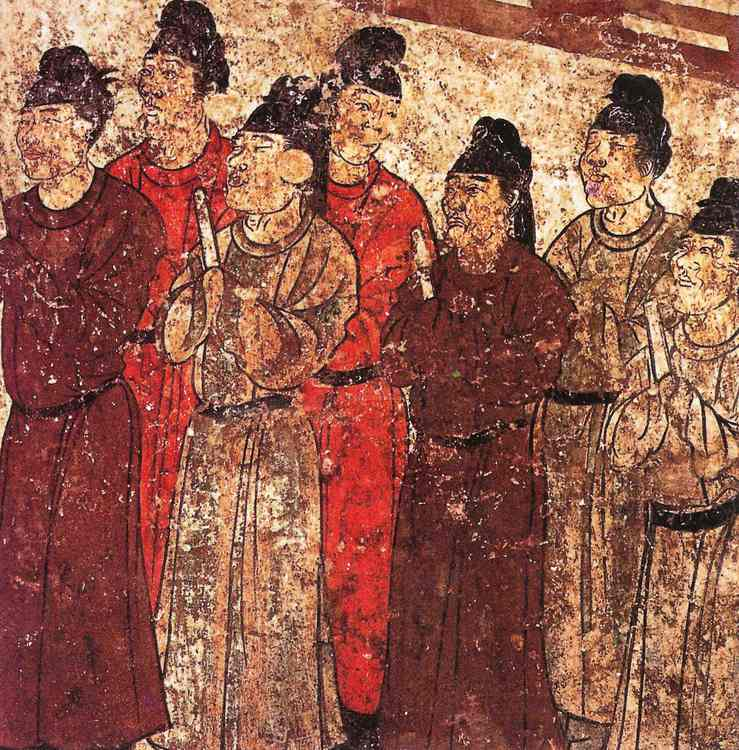
\includegraphics[width=\textwidth]{Eunuchs-in-ancient-China.jpg}
    \caption{Palace eunuchs in ancient China}
  \end{subfigure}
  \hfill
  \begin{subfigure}{0.4\textwidth}
    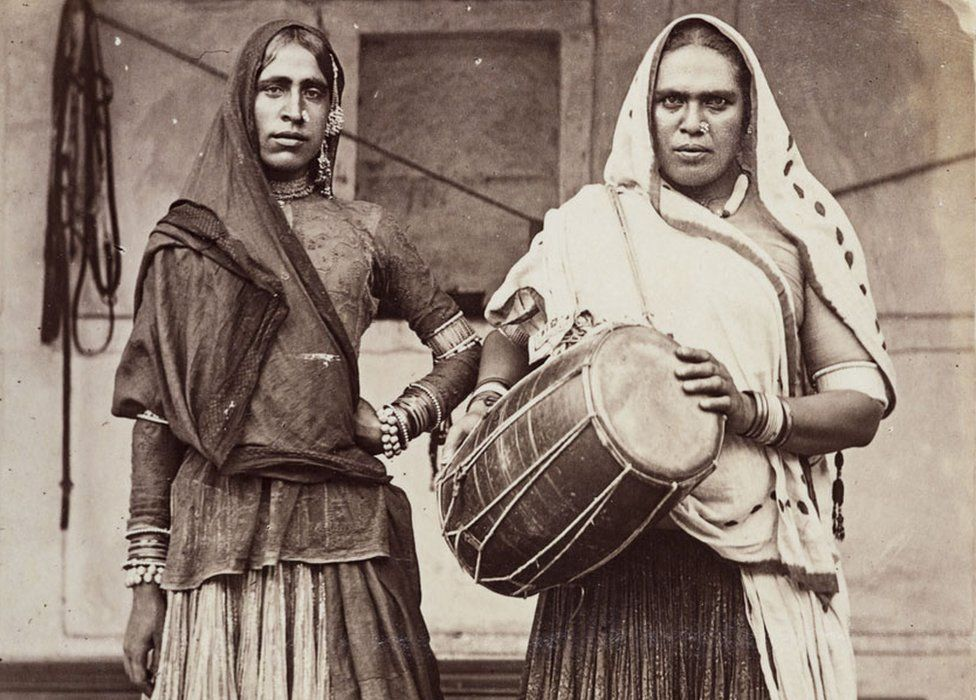
\includegraphics[width=\textwidth]{hijra.jpg}
    \caption{Hijra in India}
  \end{subfigure}
\setcounter{figure}{0}
\captionof{figure}{}
\label{eunuchs}
\end{figure}

It is in the later commentaries that we find more of a description in the form of the five types of {\em paṇḍakas}. But this also causes further confusion because the concept in its entirety did not seem to be known to the translators of the Chinese texts so they used words they knew from their own culture. There the word {\em paṇḍaka} was first translated as `impotent' (種不能男) and later as `eunuch' (黃門). The translation `eunuch' however was taken from the word `yellow gate', denoting the Han Dynasty imperial palace eunuchs. This was possibly the only way that the Chinese could relate to a {\em paṇḍaka}, being unfamiliar with the rich religious concept that they embody. It is clear that the Chinese palace eunuchs cannot be compared to the {\em hijras} from India, who are most likely the closest modern-day representative of what the {\em paṇḍakas} would have been (see figure \ref{eunuchs}).

The concept of {\em paṇḍaka} does not allow itself to be reduced to a mere word to make it acceptable and understandable for the rational mind. As Serena Nanda argues: ``Whereas Westerners feel uncomfortable with the ambiguities and contradictions inherent in such in-between categories as transvestism, homosexuality, hermaphroditism, and transgenderism, and make strenuous attempts to resolve them, Hinduism not only accommodates such ambiguities, but also views them as meaningful and even powerful.\footnote{See \cite{nanda} page 20. Note that since the time Serena Nanda wrote this passage our understanding and vocabulary of sex, sexuality and gender has changed and terms like `transvestism', `homosexuality' and `hermaphroditism' are no longer in use.}'' It is the divine representation of the feminine within the masculine. It is the human representation of the mythical tales which have deep psychological roots, namely the ambivalence that leads to the inner struggle between man's love of the feminine and his fear thereof. The concept of {\em paṇḍaka} does not match any contemporary notions. The closest representation of this term in today's world is possibly the {\em hijra}.
